\documentclass{beamer}

\usepackage{minted}

\newminted{rust}{bgcolor=bg}
\newminted{sql}{bgcolor=bg}

\AtBeginSection[]{
    \begin{frame}
        \begin{center}
            \usebeamerfont{title}\secname
        \end{center}
    \end{frame}
}

\AtBeginSubsection[]{
    \begin{frame}
        \begin{center}
            \usebeamerfont{subtitle}\subsecname
        \end{center}
    \end{frame}
}

\title{Rust-Postgres}
\subtitle{An idiomatic, native Postgres driver}
\author[sfackler]{Steven Fackler - sfackler}
\date{July 31, 2014}

\begin{document}
\definecolor{bg}{rgb}{.95,.95,.95}

\begin{frame}
\titlepage
\end{frame}

\begin{frame}{Outline}
    \tableofcontents
\end{frame}

\section{Background}

\begin{frame}{PostgreSQL}
	
\includegraphics[height=2cm]{postgres_logo.pdf}

	\begin{quote}
		``PostgreSQL is a powerful, open source object-relational database system. It has more than 15 years of active development and a proven architecture that has earned it a strong reputation for reliability, data integrity, and correctness.''
	\end{quote}
\end{frame}

\begin{frame}{Rust-Postgres}
    \begin{itemize}
        \item Started just over a year ago as ``rust-sql''.
        \item libsqlite and libpq wrappers with an eye towards a common API.
        \item Quickly renamed to ``rust-postgres'' and shifted focus to a native Postgres driver.
    \end{itemize}
\end{frame}

\section{Overview}
\subsection{Usage}

\begin{frame}[fragile]{Connecting}
	Connect with a standard psql-style URI:
	\begin{rustcode}
use postgres::{PostgresConnection, NoSsl};
let url = "postgresql://name@localhost:15410/mydb";
let conn = try!(
        PostgresConnection::connect(url, &NoSsl));
	\end{rustcode}	
	Unix sockets are supported as well:
	\begin{rustcode}
use postgres::{PostgresConnection, NoSsl};
let url = "postgresql://name@%2Frun%2Fpostgres/mydb";
let conn = try!(
        PostgresConnection::connect(url, &NoSsl));
	\end{rustcode}	
\end{frame}

\begin{frame}[fragile]{Connecting}
	Alternatively, pass a `PostgresConnectParams' struct:
	\begin{rustcode}
use postgres::{PostgresConnection, NoSsl,
               PostgresConnectParams, TargetUnix};
let params = PostgresConnectParams {
    target: TargetUnix(Path::new("/run/postgres")),
    port: Some(1234),
    .....
};
let conn = try!(
        PostgresConnection::connect(params, &NoSsl));
	\end{rustcode}
\end{frame}

\begin{frame}[fragile]{Statement Preparation}
    Queries must first be \emph{prepared} before they can be executed.

    They may be parameterized. Parameters are denoted by \verb!$n!, and are
    1-indexed.
    \begin{rustcode}
let query = "SELECT name, height
             FROM people
             WHERE age < $1";
let stmt = try!(conn.prepare(query));
    \end{rustcode}
\end{frame}

\begin{frame}[fragile]{Execution}
    The \verb!execute! method takes a slice of values to bind to the query
    parameters and returns the number of rows modified.
    \begin{rustcode}
let query = "UPDATE users SET name = $1
                WHERE age = $2";
let stmt = try!(conn.prepare(query));
let rows_updated = try!(
        stmt.execute([&"Steven", &Some(24i32)]));
    \end{rustcode}
\end{frame}

\begin{frame}[fragile]{Querying}
    \verb!query! is similar to \verb!execute! but it returns an iterator over
    the rows returned by a query. Columns may be accessed by index or name.
    \begin{rustcode}
let query = "SELECT name, age FROM users
                WHERE age < $1";
let stmt = try!(conn.prepare(query));
for row in try!(stmt.query([&18i32])) {
    let name: String = row.get(0u);
    let age: Option<i32> = row.get("age");
    println!("{} is {}", name, age);
}
    \end{rustcode}
\end{frame}

\begin{frame}[fragile]{Parameterization}
    \begin{center}
        Use it. Seriously.

        \vspace{.75cm}

        \href{http://xkcd.com/327/}{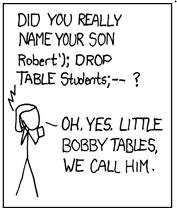
\includegraphics[height=4cm]{bobby_tables.jpg}}
    \end{center}
\end{frame}

\begin{frame}[fragile]{Transactions}
    Transactions are managed by the \verb!PostgresTransaction! object:
    \begin{rustcode}
let trans = try!(conn.transaction());
let stmt = try!(trans.prepare(...));
....

if the_coast_is_clear {
    trans.set_commit();
}

try!(trans.finish()); // COMMIT / ROLLBACK here
    \end{rustcode}
\end{frame}

\begin{frame}[fragile]{Error Handling}
    \begin{sqlcode}
CREATE TABLE foo (
    id SERIAL PRIMARY KEY,
    name VARCHAR,
    CONSTRAINT uk_foo_name UNIQUE (name))
    \end{sqlcode}
    \begin{rustcode}
let query = "INSERT INTO foo (name) VALUES ($1)";
match conn.execute(query, [&name]) {
    Err(PgDbError(PostgresDbError {
        code: UniqueViolation,
        constraint: Some(ref c),
        ..
    })) if c.as_slice() == "uk_foo_name" =>
        // Duplicate username
    _ => ...
}
    \end{rustcode}
\end{frame}

\subsection{Design}

\begin{frame}[fragile]{High Level}
    \begin{itemize}
        \item Manage resources via RAII objects.
        \item Borrowed references ensure that resources are cleaned up in the right order without the need for reference counting or garbage collection.
        \item Avoid failure in most cases - propogate errors via \verb!Result!.
        \begin{itemize}
            \item Removal of failure throughout the library cut the size of the rlib by ~50\%!
        \end{itemize}
    \end{itemize}
\end{frame}

\begin{frame}[fragile]{Strict Typing}
    Like Rust itself, Rust-Postgres won't perform implicit type conversions. A
    Postgres type is only convertable to an ``equivalent'' Rust type and vice
    versa.
    \begin{sqlcode}
CREATE TABLE foo (id INT PRIMARY KEY, bar BIGINT) 
    \end{sqlcode}
    \begin{rustcode}
let stmt = try!conn.prepare("SELECT id FROM foo"));
for row in try!(stmt.query([])) {
    row.get::<i32>(0u); // ok
    row.get::<Option<i32>>(0u); // ok
    row.get::<uint>(0u); // not ok
}

let stmt = try!(
        conn.prepare("UPDATE foo SET bar = $1"));
try!(stmt.execute([&1i64])); // ok
try!(stmt.execute([&None::<i64>])); // ok
try!(stmt.execute([&"1"])); // not ok
    \end{rustcode}
\end{frame}

\begin{frame}{Extensibility}
    Postgres allows for extensions which define new types and operations.
    \begin{itemize}
        \item PostGIS
        \item HStore
        \item etc
    \end{itemize}

    Rust-Postgres provides an extendible API for conversions to and from
    Postgres values.
\end{frame}

\begin{frame}[fragile]{Type Conversion}
    All conversions are done through two traits
    \begin{rustcode}
pub trait ToSql {
    fn to_sql(&self, ty: &PostgresType)
              -> PostgresResult<(Format,
                                 Option<Vec<u8>>)>;
} 

pub trait FromSql {
    fn from_sql(ty: &PostgresType,
                raw: &Option<Vec<u8>>)
                -> PostgresResult<Self>;
}
    \end{rustcode}
\end{frame}

\subsection{Macros}

\begin{frame}[fragile]{Compile Time Checks}
    Compile time checks are awesome, but SQL opens up a series of issues that
    won't be discovered until runtime.
    \begin{itemize}
        \item Invalid syntax
        \begin{sqlcode}
SELECT * FORM foo 
        \end{sqlcode}
        \item Parameter count mismatch
        \begin{rustcode}
try!(conn.execute("UPDATE foo SET a = $1
                        WHERE b = $2",
                  [&1i32]));
        \end{rustcode}
        \item Schema mismatch
        \begin{sqlcode}
SELECT nmae FROM users
        \end{sqlcode}
    \end{itemize}
\end{frame}

\begin{frame}[fragile]{Syntax Extensions to the Rescue}
    Link against PostgreSQL's query parser and have it do the heavy lifting!
    \begin{rustcode}
#[phase(plugin)]
extern crate postgres_macros;

let query = sql!("SELECT * FORM foo");
    \end{rustcode}
    \begin{verbatim}
test.rs:8:18: 8:35 error: Invalid syntax at
    position 10: syntax error at or near "FORM"
test.rs:8     let query = sql!("SELECT * FORM foo");
                               ^~~~~~~~~~~~~~~~~~~
    \end{verbatim}
\end{frame}

\begin{frame}[fragile]{Syntax Extensions to the Rescue}
    \begin{rustcode}
#[phase(plugin)]
extern crate postgres_macros;

try!(execute!(conn,
              "UPDATE foo SET a = $1
                WHERE b = $2",
              &1i32));
    \end{rustcode}
    \begin{verbatim}
test.rs:7:1: 10:23 error: Expected 2 query parameters
        but got 1
test.rs:7 try!(execute!(conn,
test.rs:8               "UPDATE foo SET a = $1
test.rs:9                 WHERE b = $2",
test.rs:10               &1i32));
    \end{verbatim}
\end{frame}

\section{Future}

\begin{frame}{What's Missing}
    Rust-Postgres defines the basics, but much of the infrastructure on top
    is still missing.
    \begin{itemize}
        \item Connection Pool - There is a pool in Rust-Postgres but it's nowhere near sufficient. \href{https://github.com/sfackler/rust-postgres/issues/44}{sfackler/rust-postgres\#44}
        \item ORM - Syntax extensions could allow for an interesting ORM system. \href{https://github.com/sfackler/rust-postgres/issues/47}{sfackler/rust-postgres\#47}
    \end{itemize}
\end{frame}

\begin{frame}{That's It!}
    \begin{center}
        Questions?

        \vspace{10mm}

        \url{https://github.com/sfackler/rust-postgres}
    \end{center}
\end{frame}

\end{document}
